%\chapter{Adding interaction to Bayesian nonparametric hierarchical clustering}

\section{Motivation}
Clustering is a basic tool of exploratory data analysis. There are a variety of efficient algorithms---including $k$-means, EM for Gaussian mixtures, and hierarchical agglomerative schemes---that are widely used for discovering ``natural'' groups in data. Unfortunately, they don't always find a grouping that suits the user's needs.

This is inevitable. In any moderately complex data set, there are many different plausible grouping criteria. Should a collection of rocks be grouped according to value, or shininess, or geological properties? Should animal pictures be grouped according to the Linnaean taxonomy, or cuteness? Different users have different priorities, and an unsupervised algorithm has no way to magically guess these.

As a result, a rich body of work on {\it constrained} clustering has emerged.
In this setting, a user supplies guidance, typically in the form of ``must-link'' or ``cannot-link'' constraints, pairs of points that must be placed together or apart. Introduced by \citet{Wagstaff2001}, these constraints have since been incorporated into many different {\it flat} clustering procedures~\citep{Wagstaff2000,Bansal2004,Basu2004,Kulis2009,Biswas2014}.

In this chapter, we introduce constraints to {\it hierarchical clustering}, the recursive partitioning of a data set into successively smaller clusters to form a tree. A hierarchy has several advantages over a flat clustering. First, there is no need to specify the number of clusters in advance. Second, the tree captures cluster structure at multiple levels of granularity, simultaneously. As such, trees are particularly well-suited for exploratory data analysis and the discovery of natural groups.

There are several well-established methods for hierarchical clustering, the most prominent among which are the bottom-up agglomerative methods such as average linkage (see, for instance, Chapter 14 of \citet{Hastie2009}). But they suffer from the same problem of under-specification that is the scourge of unsupervised learning in general. And, despite the rich literature on incorporating additional guidance into flat clustering, there has been relatively little work on the hierarchical case.

What form might the user's guidance take? The usual must-link and cannot-link constraints make little sense when data has hierarchical structure. Among living creatures, for instance, should {\tt elephant} and {\tt tiger} be linked? At some level, yes, but at a finer level, no. A more straightforward assertion is that {\tt elephant} and {\tt tiger} should be linked in a cluster that does not include {\tt snake}. We can write this as a {\it triplet} $(\{\mbox{\tt elephant}, \mbox{\tt tiger}\}, \mbox{\tt snake})$. We could also assert $(\{\mbox{\tt tiger}, \mbox{\tt leopard}\}, \mbox{\tt elephant})$. Formally, $(\{a,b\},c)$ stipulates that the hierarchy contains a subtree (that is, a cluster) containing $a$ and $b$ but not $c$.

A wealth of research addresses learning taxonomies from triplets {\it alone}, mostly in the field of phylogenetics: see \citet{Felsenstein2004} for an overview, and \citet{Aho1981} for a central algorithmic result. Let's say there are $\numdata$ data items to be clustered, and that the user seeks a particular hierarchy $\tree^*$ on these items. This $\tree^*$ embodies at most ${\numdata \choose 3}$ triplet constraints, possibly less if it is not binary. It was pointed out in \citet{Tamuz2011} that roughly $\numdata \log \numdata$ carefully-chosen triplets are enough to fully specify $\tree^*$ if it is balanced. This is also a lower bound: there are $\numdata^{\Omega(\numdata)}$ different labeled rooted trees, so each tree requires $\Omega(\numdata \log \numdata)$ bits, on average, to write down---and each triple provides $O(1)$ bits of information, since there are just three possible outcomes for each set of points $a,b,c$. Although $\numdata \log \numdata$ is a big improvement over $\numdata^3$, it is impractical for a user to provide this much guidance when the number of points is large. In such cases, a hierarchical clustering cannot be obtained on the basis of constraints alone; the geometry of the data must play a role.

We consider an interactive process during which a user incrementally adds constraints.
\begin{itemize}
\item Starting with a pool of data $\data \subseteq \R^\d$, the machine builds a candidate hierarchy $\tree$.
\item The set of constraints $C$ is initially empty.
\item Repeat:
\begin{itemize}
\item The machine presents the user with a small portion of $\tree$: specifically, its restriction to $O(1)$ leaves $S \subset X$. We denote this $\tree|_S$.
\item The user either accepts $\tree|_S$, or provides a triplet constraint $(\{a,b\},c)$ that is violated by it.
\item If a triplet is provided, the machine adds it to $C$ and modifies the tree $T$ accordingly.
\end{itemize}
\end{itemize}
In realizing this scheme, a suitable clustering algorithm and querying strategy must be designed. Similar issues have been confronted in flat clustering---with must-link and cannot-link constraints---but the solutions are unsuitable for hierarchies, and thus a fresh treatment is warranted.

\subsubsection*{The clustering algorithm}

What is a method of hierarchical clustering that takes into account the geometry of the data points as well as user-imposed constraints? 

We adopt an \emph{interactive Bayesian} approach. The learning procedure is uncertain about the intended tree and this uncertainty is captured in the form of a distribution over all possible trees. Initially, this distribution is informed solely by the geometry of the data but once interaction begins, it is also shaped by the growing set of constraints.

The nonparametric Bayes literature contains a variety of different distributional models for hierarchical clustering. We describe a general methodology for extending these to incorporate user-specified constraints. For concreteness, we focus on the Dirichlet diffusion tree~\citep{Neal2003}, which has enjoyed empirical success. We show that triplet constraints are quite easily accommodated: when using a Metropolis-Hastings sampler, they can efficiently be enforced, and the state space remains strongly connected, assuring convergence to the unique stationary distribution.

\subsubsection*{The querying strategy}

What is a good way to select the subsets $S$? A simple option is to pick them at random from $\data$. We show that this strategy leads to convergence to the target tree $\tree^*$. Along the way, we define a suitable distance function for measuring how close $\tree$ is to $\tree^*$. 

%This allows us to give a simple rule for when to stop querying if we seek a tree $\epsilon$-close to the target.

We might hope, however, that a more careful choice of $S$ would lead to faster convergence, in much the same way that intelligent querying is often superior to random querying in active learning. In order to do this, we show how the Bayesian framework allows us to quantify which portions of the tree are the most uncertain, and thereby to pick $S$ that focuses on these regions.

Querying based on uncertainty sounds promising, but is dangerous because it is heavily influenced by the choice of prior, which is ultimately quite arbitrary. Indeed, if only such queries were used, the interactive learning process could easily converge to the wrong tree. We show how to avoid this situation by interleaving the two types of queries.

Finally, we present a series of experiments that illustrate how a little interaction leads to significantly better hierarchical clusterings.


\subsection{Other related work}

A related problem that has been studied in more detail~\citep{Zoller2000,Eriksson2011,Krishnamurthy2012} is that of building a hierarchical clustering where the only information available is pairwise similarities between points, but these are initially hidden and must be individually queried.

In another variant of interactive flat clustering~\citep{Balcan2008,Awasthi2010,Awasthi2013}, the user is allowed to specify that individual clusters be merged or split. A succession of such operations can always lead to a target clustering, and a question of interest is how quickly this convergence can be achieved.

Finally, it is worth mentioning the use of triplet constraints in learning other structures, such as Euclidean embeddings~\citep{Borg1997}.

\iffalse
\section{Bayesian hierarchical clustering}
%\subsection{Priors on trees}

\fi
\section{Adding interaction}

Impressive as Bayesian nonparametric hierarchical clustering is, there is no reason to suppose that it will magically find a tree that suits the user's needs. But a little interaction can be helpful in improving the outcome.

Let $\tree^*$ denote the target hierarchical clustering. It is not necessarily the case that the user would be able to write this down explicitly, but this is the tree that captures the distinctions he/she is able to make, or wants to make. Figure~\ref{fig:refinement} (left) shows an example, for a small data set of 5 points. In this case, the user does not wish to distinguish between points $1,2,3$, but does wish to place them in a cluster that excludes point $4$.

We could posit our goal as exactly recovering $\tree^*$. But in many cases, it is good enough to find a tree that captures all the distinctions within $\tree^*$ but also possibly has some extraneous distinctions, as in the right-hand side of Figure~\ref{fig:refinement}.

\begin{figure}
    \centering
    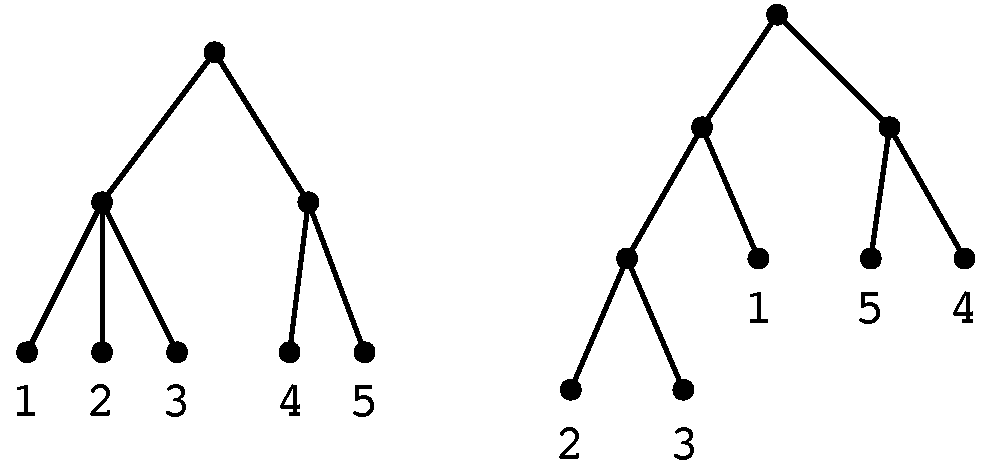
\includegraphics[width=3in]{img/ibhc/refinement.pdf}
    \caption{Target tree $T^*$ (left) and a refinement of it.}
    \label{fig:refinement}
\end{figure}

Formally, given data set $\data$, we say $S \subseteq \data$ is a {\it cluster} of tree $\tree$ if there is some node of $\tree$ whose descendant leaves are exactly $S$. We say $\tree$ is a {\it refinement} of $\tree^*$ if they have the same set of leaves, and moreover every cluster of $\tree^*$ is also a cluster of $\tree$. This, then, is our goal: to find a refinement of the target clustering $\tree^*$.

\subsection{Triplets}

The user provides feedback in the form of triplets. The constraint $(\{a,b\},c)$ means that the tree should have a cluster containing $a$ and $b$ but not $c$. Put differently, the lowest common ancestor of $a,b$ should be a strict descendant of the lowest common ancestor of $a,b,c$.

Let $\Delta(\tree)$ denote the set of all proper triplet constraints embodied in tree $\tree$. If $\tree$ has $n$ nodes, then $|\Delta(\tree)| \leq {n \choose 3}$. For non-binary trees, it will be smaller than this number. Figure~\ref{fig:refinement} (left), for instance, has no triplet involving $1,2,3$. 

Refinement can be characterized in terms of triplets.
\begin{restatable}{lemma}{treerefinement}
\label{thm:treerefinement}
Tree $\tree$ is a refinement of tree $\tree'$ if and only if $\Delta(\tree') \subseteq \Delta(\tree)$.
\end{restatable}
\begin{proof}
See supplement.
\end{proof}
In particular, {\it any triplet-querying scheme that converges to the full set of triplets of the target tree $\tree^*$ is also guaranteed to produce trees that converge to a refinement of $\tree^*$.}

With this lemma in mind, it is natural to measure how close a tree $\tree$ is to the target $\tree^*$ with the following (asymmetric) distance function, which we call {\it triplet distance} (TD):

%\subsection{Triplet Distance}
%To better understand the performance of clustering algorithm
%and the various triplet querying schemes,
%we first define a distance function between
%a candidate tree and the desired tree.

%$T$ is defined to be a \emph{refinement} of $T^*$ if
%if every cluster of $T^*$ is in $T$.
%In the general setting, $T^*$ may be a $k$-ary tree
%and our algorithm only produces a binary tree. 
%For example, in a $K$-way classification problem, the desired
%tree $T^*$ would be a root node with $K$ children corresponding to %each class. 
%Each of these $K$ children would have all data belonging to its class %as
%a child. See \autoref{fig:kway} for an example. 

%If a binary tree $T$ is a refinement of $T^*$ in the $K$-way
%classification problem,
%there exist nodes in $T$ that contain
%solely the data for each class and this is the closest binary tree we
%can obtain.
%Thus, we desire a distance function such that if $T$ is a refinement
%of $T^*$, their distance should be 0.

%\begin{figure}[H]
%    \centering
%    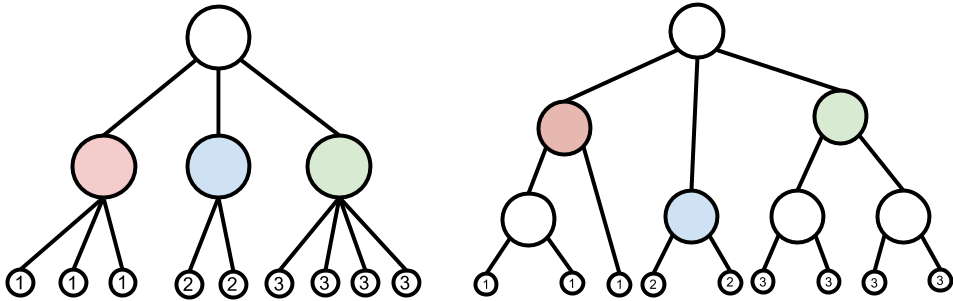
\includegraphics[width=0.5\textwidth]{img/ibhc/KWayTree}
%    \caption{A 4-way classification tree on the left
%    and a refinement of it on the right. Nodes
%    with matching colors represent matching clusters.}
%    \label{fig:kway}
%\end{figure}

%Let $\mathcal{C}(T)$ be the enumeration of all triplets
%satisfied by tree $T$.
%For a given desired \emph{master tree} $T^*$
%the triplet distance (TD) between $T^*$ and a candidate tree $T$
%is

\begin{align}
    \mathrm{TD}(\tree^*, \tree) = \frac{\sum_{c \in \Delta(\tree^*)} \mathbb{I}(c \notin \Delta(\tree)) }{|\Delta(\tree^*)|}
\end{align}
where $\mathbb{I}$ is the indicator function.
% Lemma
%If $T$ is a refinement of $T^*$, their triplet distance is zero
%as $\mathcal{C}(T^*) \subseteq \mathcal{C}(T)$.
This distance is zero exactly when $\tree$ is a refinement of $\tree^*$, in which case we have reached our goal. 

%User guidance can assist in under-specified
%unsupervised learning problems. We now
%provide a concrete means of obtaining 
%information about hierarchical structure in data
%from a user, in the form of \emph{triplet feedback}.

%For hierarchies, a triplet is a set of data
%of the form $(\{a, b\}, c)$, such that
%$a$ and $b$ should belong in a subtree
%together without $c$. Let $\text{lca}(u, v)$ be
%the lowest common ancestor of nodes $u$ and $v$. 
%Formally, we can verify that a tree satisfies a triplet
%$(\{a, b\}, c)$ if $\text{lca}(a, b)$ is a descendant
%of both $\text{lca}(a, c)$ and $\text{lca}(b, c)$.

A simple strategy for obtaining triplets 
would be to present the user with three randomly
chosen data points and have the user pick the odd one out.
This strategy has several drawbacks.
First, some sets of three points have no triplet constraint 
(for instance, points $1,2,3$ in \autoref{fig:refinement}).
Second, the chosen set of points might correspond to a triplet
that has already been specified, or is {\it implied} by 
specified triplets. For example, knowledge of $(\{a, b\}, c)$ and
$(\{b, c\}, d)$ implies $(\{a, c\}, d)$.
Enumerating the set of implied
triplets is non-trivial for $n > 3$ triplets~\citep{Bryant1995},
making it difficult to avoid these implied triplets
in the first place.

We thus consider another strategy---rather
than the user arranging three data points into
a triplet, the user observes
the hierarchy induced over some $O(1)$-sized
subset $S$ of the data and corrects
an error in the tree by supplying a triplet.
We call this is a \emph{subtree query}.
Finally, we note that in this work
we only consider the \emph{realizable} case
where the triplets obtained
from a user do not contain contradictory information
and that there is a tree that satisfies
all of them.

%\subsection{Triplet feedback on subtrees}
%The interactive process integrates
%user feedback into a hierarchy
%after querying the user for a triplet.
%We perform this query by
%showing a user the subtree
%over a particular subset of data
%and ask to either
%accept the subtree as correct, or
%report a triplet that is violated by
%the subtree.
%
%Formally, given a candidate hierarchy $T$
%that satisfies a set of triplets $C$ ,
%we first obtain some $O(1)$ size
%subset of the dataset  $S \subset X$,
%and find the induced subtree
%$T|_S$.
%$T|_S$ is shown to a user whereupon
%the user can either accept the tree,
%acknowledging that there are no errors in its
%structure, or report a triplet
%$(\{a, b\}, c)$ that is violated by this subtree.

%This approach confers several benefits over
%the simple approach of selecting three points
%at random. Subtree queries have the benefit
%of never returning a triplet 
%implied by $C$. A tree that satisfies $C$
%will by definition will satisfy all of $C$'s
%implied triplets. 
%In addition,
%the triplet reported by the user
%is likely to be more informative
%as the triplet corresponds to an 
%error in a candidate hierarchy.
%However, this method assumes
%the existence of an algorithm
%that can produce candidate trees
%that satisfy $C$.

\subsection{Finding a tree consistent with constraints}
\label{sec:aho}
We start with a randomly initialized hierarchy $\tree$
over our data
and show an induced subtree $\tree|_S$ to the user, obtaining the
first triplet. The next step is constructing  
a new tree that satisfies the triplet.
This begins the feedback cycle; a user provides a triplet
given a subtree and the triplet is incorporated into a clustering algorithm,
producing a new candidate tree.
A starting point is 
an algorithm that returns 
a tree consistent with a set of triplets.

The simplest algorithm to solve this problem is
the \texttt{BUILD} algorithm, introduced in \citet{Aho1981}.
Given a set of triplets $C$, \texttt{BUILD}
will either return a tree that satisfies $C$, or error 
if no such tree exists.
In \texttt{BUILD}, we first construct the {\it Aho graph}
$G_C$, which has a vertex for each data point and an 
undirected edge $\{a,b\}$ for each triplet constraint $(\{a,b\},c)$.
If $G_C$ is connected, there is no tree that satisfies all
triplets. Otherwise, the top split of the tree is a partition of 
the connected components of $G_C$: any split is fine as long as 
points in the same component stay together. Satisfied triplets are discarded, and \texttt{BUILD} then continues recursively on the
left and right subtrees.

\texttt{BUILD} satisfies triplet constraints but ignores 
the geometry of the data, whereas we wish to take both into
account. By incorporating triplets into the posterior DDT 
sampler, we obtain high likelihood trees that still satisfy $C$.


\subsection{Incorporating triplets into the sampler}

In this section, we present an algorithm
to sample candidate trees 
from the posterior DDT, constrained
by a triplet set $C$.
It is based on the subtree prune and regraft move.
%The Metropolis-Hastings algorithm for the DDT
%alternates sampling tree structure
%via SPR moves and latent divergence locations
%via Gibbs Sampling.
%This process produces tree samples
%that converge to the posterior
%distribution of the DDT
%given data.

\begin{figure*}[htp!]
    \centering
    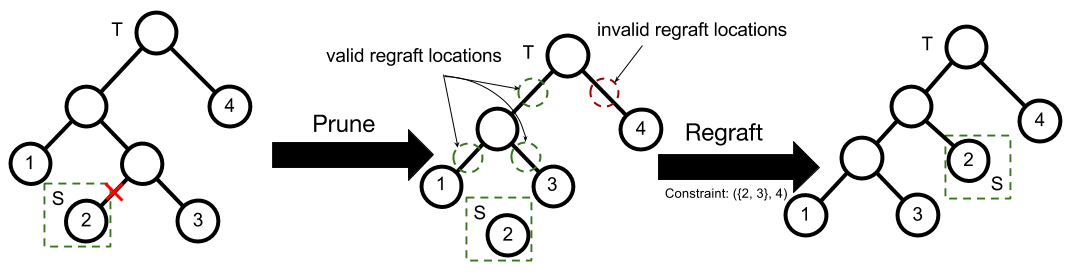
\includegraphics[width=\textwidth]{img/ibhc/ConstrainedSPRMove}
    \caption{
            Visualized is a constrained-SPR move.
            Pruning is identical  but
            a regraft location is selected from the valid regraft locations
            limited by triplets.
            In this image, we are constrained by the sole triplet $(\{2, 3\}, 4)$.
            }
    \label{fig:constrainedsprmove}
\end{figure*}

The SPR move is of particular interest
because we can efficiently
enforce triplets to form a \emph{constrained-SPR move},
resulting in a sampler
that only produces trees that satisfy a set of triplets.
A \emph{constrained-SPR move} is defined as
an SPR move that assigns zero probability to
any resulting trees that would violate a set of triplets.
Restricting the neighborhood of an SPR move
runs the risk of partitioning the state space,
losing the convergence
guarantees of the Metropolis-Hastings algorithm.
Fortunately, a constrained-SPR move does not compromise
strong connectivity.
For any realizable triplet set $C$,
we prove 
the constrained-SPR move Markov chain's aperiodicity and irreducibility.

Consider the Markov chain on the state space 
of rooted binary trees that is induced by the constrained sampler.
%\subsection{Proof of \autoref{thm:apr}}
\begin{restatable}{lemma}{aperiodic}
The constrained-SPR Markov chain is aperiodic.
\end{restatable}
\begin{proof}
A sufficient condition for aperiodicity
is the existent of a ``self-loop'' in the transition matrix: a non-zero probability of a state transitioning to itself.
Supposed we have pruned a subtree already.
When regrafting, the ordinary SPR move
has a non-zero probability of choosing any branch,
and a constrained-SPR move cannot regraft
to branches that would violate triplets.
Since the current tree in the Markov chain
satisfies triplet set $C$, there is a non-zero probability
of regrafting to the same location. 
We thus have an aperiodic Markov chain.
\end{proof}



%\subsection{Proof of \autoref{thm:irr}}
%\label{app:irr}
%\irreducible*
\begin{restatable}{lemma}{irreducible}
\label{thm:irr}
A constrained-SPR Markov chain is irreducible.
\end{restatable}

\begin{proof}
(sketch) To show irreducibility,
we show that a tree $\tree$ has an non-zero
probability of reaching an arbitrary tree
$\tree'$ via constrained-SPR moves where
both $\tree$ and $\tree'$ satisfy a set of triplets $C$.
Our proof strategy
is to construct a canonical tree 
$\tree_C$, and show that there exists
a non-zero probability path from $\tree$ to $\tree_C$,
and therefore from $\tree'$ to $\tree_C$.
We then show that for a given constrained-SPR move,
the reverse move has a non-zero probability.
Thus, there exists a path from $\tree$ to $\tree_C$ to
$\tree'$, satisfying irreducibility.

Recall that the split at a node in a binary
tree that satisfies triplet set $C$
corresponds to a binary partition
of the Aho graph at the node (see Section \ref{sec:aho}).
$\tree_C$ is a tree such that
every node in $\tree_C$ is in \emph{canonical form}.
A node is in canonical form if it is a leaf node,
or, the partition of the Aho graph
at that node can be written as $(l, r)$.
$l$ is the single connected component
containing the point with the minimum data index,
and $r$ is the rest of the components.

To convert a particular node $s$ into canonical form,
we first perform ``grouping'',
which puts $l$ into a single descendant of $s$
via constrained-SPR moves.
We then make two constrained-SPR moves to convert
the partition at $s$ into the form $(l, r)$ (see \autoref{fig:canonical}).
We convert all nodes into canonical form recursively, turning 
an arbitrary tree $\tree$ into $\tree_C$.

Finally, the reverse constrained-SPR move has a non-zero
probability. Suppose
we perform a constrained-SPR move on tree $\tree_1$, converting it into $\tree_2$ by 
detaching subtree $s$
and attaching it to branch $(u, v)$.
A constrained-SPR move on $\tree_2$ can select
$s$ for pruning 
and can regraft it to form $\tree_1$ with a non-zero
probability since
$\tree_1$ satisfies the same constraint set as $C$.
For a full proof, please refer to the supplement.
\end{proof}

\begin{figure*}
    \centering
    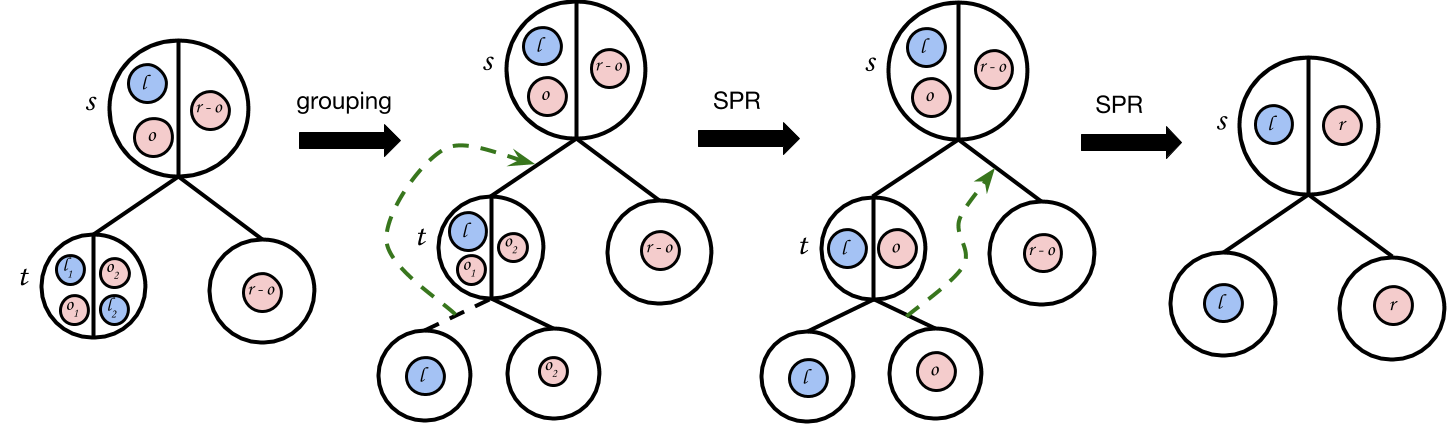
\includegraphics[width=\textwidth]{img/ibhc/CanonicalTree}
    \caption{The process of converting $s$ into canonical form.
    We first group nodes from $l$ into their own isolated subtree, then perform
    two constrained-SPR moves to put $s$ into canonical form.}
    \label{fig:canonical}
\end{figure*}

%\begin{restatable}{lemma}{aperiodic}
%\label{thm:apr}
%\end{restatable}
%\begin{proof} See \ref{app:apr}.
%\end{proof}
%
%\begin{restatable}{lemma}{irreducible}
%\label{thm:irr}
%A constrained-SPR Markov chain is irreducible.
%\end{restatable}
%\begin{proof} See \ref{app:irr}.
%\end{proof}


The simplest possible scheme for a constrained-SPR move 
would be rejection sampling. The Metropolis-Hastings
algorithm for the DDT would be the same as in the
unconstrained case,
but any trees violating $C$ would have accept
probability $0$. Although this procedure is correct,
it is impractical. As the number of triplets
grows larger, more trees will be rejected
and the sampler will slow down over time.

To efficiently sample a tree that satisfies a set of triplets $C$, 
we modify the regraft in the ordinary SPR move. 
The constrained-SPR move must assign zero probability
to any regraft branches that would result in a tree
that violates $C$.
This is accomplished by generating the path from the root
in the same manner as sampling a branch,
but avoiding paths that would resulted in violated triplets.


\subsubsection*{Description of constrained-SPR sampler}
%The pruning procedure for the constrained-SPR sampler
%is identical to the unconstrained pruning procedure.
%Sampling a valid regraft location, however, involves
%eliminating all possible locations that would
%result in violated triplets. For the DDT,
%this can be accomplished by modifying
%the generative process used to sample regraft branches.

Recall that in the DDT's sampling procedure for regraft branches,
a particle at a node picks a branch, and either diverges from that
branch or recursively samples the node's child.
Let $s$ be the root of the subtree we are currently grafting 
back onto tree $\tree$, let $C$ be the
triplet set, and let $\texttt{leaves}(u)$
denote the descendant-leaves of node $u$.
Suppose we are are currently at node $u$,
deciding whether to diverge
at the branch $(u, v)$ or to recursively sample $v$.
Consider any triplet $(\{a, b\}, c) \in C$. If all---or none---of $a,b,c$ are in $\texttt{leaves}(s)$, then the triplet is 
unaffected by the graft, and can be ignored. Otherwise, 
some checks are needed:
\begin{enumerate}
\item $c \in \texttt{leaves}(s)$

Then we know $a,b \not\in \texttt{leaves}(s)$. If $a$ and $b$ are split across $v$'s children,
we are banned from sampling $v$.

\item $a \in \texttt{leaves}(s)$ but $b,c \not\in \texttt{leaves}(s)$

If both $b$ and $c$ are in $\texttt{leaves}(v)$, we are
required to sample $v$.
If just $c$ is in $\texttt{leaves}(v)$, we are banned
from both diverging at $(u, v)$ and sampling $v$.
Otherwise we can either diverge at $(u, v)$ or sample $v$.

\end{enumerate}

%\begin{enumerate}
%\item[1.] A node $u$ is \emph{path-banned} if for
%any triplet $(\{a, b\}, c) \in C$, 
%$(a \in \texttt{leaves}(s) \land b \notin \texttt{leaves}(u) \land c \in \texttt{leaves}(u)) \lor (b \in \texttt{leaves}(s) \land a \notin \texttt{leaves}(u) \land c \in \texttt{leaves}(u))$.
%Let $p$ be $u$'s parent.
%Intuitively, if $u$ is \emph{path-banned}, we cannot
%graft to the branch $(p, u)$, as we would automatically
%violate a triplet. This is because there is some triplet$(\{a, b\}, c)$
%in $C$ such that attaching $s$ to $(p, u)$ would result in a subtree
%that contains either $a$ and $c$ but not $b$ or $b$ and $c$ but not $a$.
%
%\item[2.] A node $u$ is \emph{sample-banned} if 
%for
%any triplet $(\{a, b\}, c) \in C$, 
%$(c \in \texttt{leaves}(s)) \land ((a \in \texttt{leaves}(v) \land b \in \texttt{leaves}(w)) \lor (a \in \texttt{leaves}(w) \land b \in \texttt{leaves}(v))$
%where $v$ and $w$ are the children of $u$. 
%Intuitively,
%this means that there exist some $a$ and $b$ in our triplet set
%that are split between $u$'s children. Attaching a subtree containing
%$c$ to a any branch below $u$ would violate a triplet.
%
%\item[3.] A node $u$ is \emph{path-required} if for
%any triplet $(\{a, b\}, c) \in C$, 
%$(a \in \texttt{leaves}(s) \land b \in \texttt{leaves}(u)) \lor (b \in \texttt{leaves}(s) \land a \in \texttt{leaves}(u))$. 
%If $u$ is \emph{path-required}, the particle must enter its branch,
%as for some triplet $(\{a, b\}, c)$, if $a$ is in our
%pruned subtree, then $b$ is in $u$ and $c$ is in $u$'s sibling.
%Choosing the branch to $u$'s sibling would violate this triplet.
%
%\item[4.] A node $u$ is \emph{sample-required} if for
%any triplet $(\{a, b\}, c) \in C$, 
%$(a \in \texttt{leaves}(s) \land b \in \texttt{leaves}(u) \land c \in \texttt{leaves}(u)) \lor (b \in \texttt{leaves}(s) \land a \in \texttt{leaves}(u) \land c \in \texttt{leaves}(u))$.
%If $u$ being \emph{sample-required} 
%means that there exists some $a$ and $c$ or $b$ and $c$
%in our triplet set that are already in a subtree in $T$ together.
%We must attach our subtree such that this triplet is not violated.
%
%\end{enumerate}
(The case where $b \in \texttt{leaves}(s)$ is
symmetric to case 2.)
If we choose to sample $v$, we remove
constraints from our current set $C$ that are now satisfied,
and continue recursively.
This defines a procedure by which we can sample
a divergence branch that does not violate constraints.

While the constrained-SPR sampler can produce
a set of trees given a set of static constraints,
the \texttt{BUILD} algorithm is useful in
adding new triplets into the sampler.
Suppose we have been sampling trees with constrained-SPR moves
with satisfying triplet set $C$ 
and we obtain a new triplet $u = (\{a, b\}, c)$ from a user query. 
We take the current tree $\tree$ and find the least common ancestor 
(call it $z$) of $a$ and $b$. We then call 
\texttt{BUILD}$(C + \{u\})$ on just the nodes in 
$\texttt{leaves}(z)$, and 
we substitute the resulting subtree at position $z$ in tree $\tree$.

\subsection{Intelligent subset queries}
We now have a method to sample a constrained
distribution over candidate trees.
Given a particular candidate tree $\tree$,
our first strategy for subtree querying
is to pick a random subset $S$ of the leaves
of constant size, and show the user
the induced subtree over the subset, $\tree|_S$.
We call this \emph{random subtree querying}.
But can we use a set of trees produced by the sampler
to make better subtree queries?
If tree structure is ambiguous in a particular region of data,
i.e. there are several hierarchies that could explain
a particular configuration of data, 
the MH algorithm will sample over
these different configurations. A query over points
in these ambiguous regions may help our algorithm
converge to a better tree faster. By looking for
these regions in our samples, we can choose query
subsets $S$ for which the tree structure is highly variable, 
and hopefully the resulting triplet from the user will 
reduce the ambiguity.

More precisely, we desire a notion of tree variance.
Given a set of trees $\trees$, what is the variance
%TODO: check this
over a given subset of the data $S$?
We propose using the notion of tree distance
as a starting point. 
For a given tree $\tree$, the tree distance between two nodes $a$ and $b$,
denoted $\texttt{treedist}_T(a, b)$,
is the number of edges of $\trees$ needed to get from $a$ to $b$.
Consider two leaves $u$ and $v$. If the tree structure around
them is static, we expect the tree distance
between $u$ and $v$ to change very little, as the surrounding tree
will not change. However, if there is
ambiguity in the surrounding structure, the tree distance will
be more variable.
Given a subset of data $S$ and a set of trees $\trees$,
the tree distance variance (TDV) of the trees over the subset is defined as:
\begin{align}
    \text{TDV}(\trees, S) = \max_{u, v \in S}\mathrm{Var}_{\tree \in \trees}[\texttt{treedist}_{\tree|_S}(u, v)]
\end{align}

This measure of variance is
the \emph{max} of the variance of tree distance between
any two points in the subset. Computing this requires
$O(|\trees||S|^2 \log|S|)$ time, and since since $|S|$ is constant,
it is not prohibitively expensive.

Given a set of trees from the sampler $\trees$,
we now select a high-variance subtree
by instantiating $L$ random subsets of constant size, $S_1, \ldots, S_L$
and picking $\text{argmax}_l \text{TDV}(\trees, S_l)$.
We call this \emph{active subtree querying}.
Although using tree variance will help reconcile ambiguity in the tree structure,
if a set of samples from a tree all violate the same triplet,
it is unlikely that active querying will recover that triplet.
Thus, interleaving random querying and active querying
will hopefully help the algorithm converge quickly, while avoiding
local optima.

\section{Experiments}

\begin{figure}
    \centering
    \begin{subfigure}[]{0.7\textwidth}
        \centering
        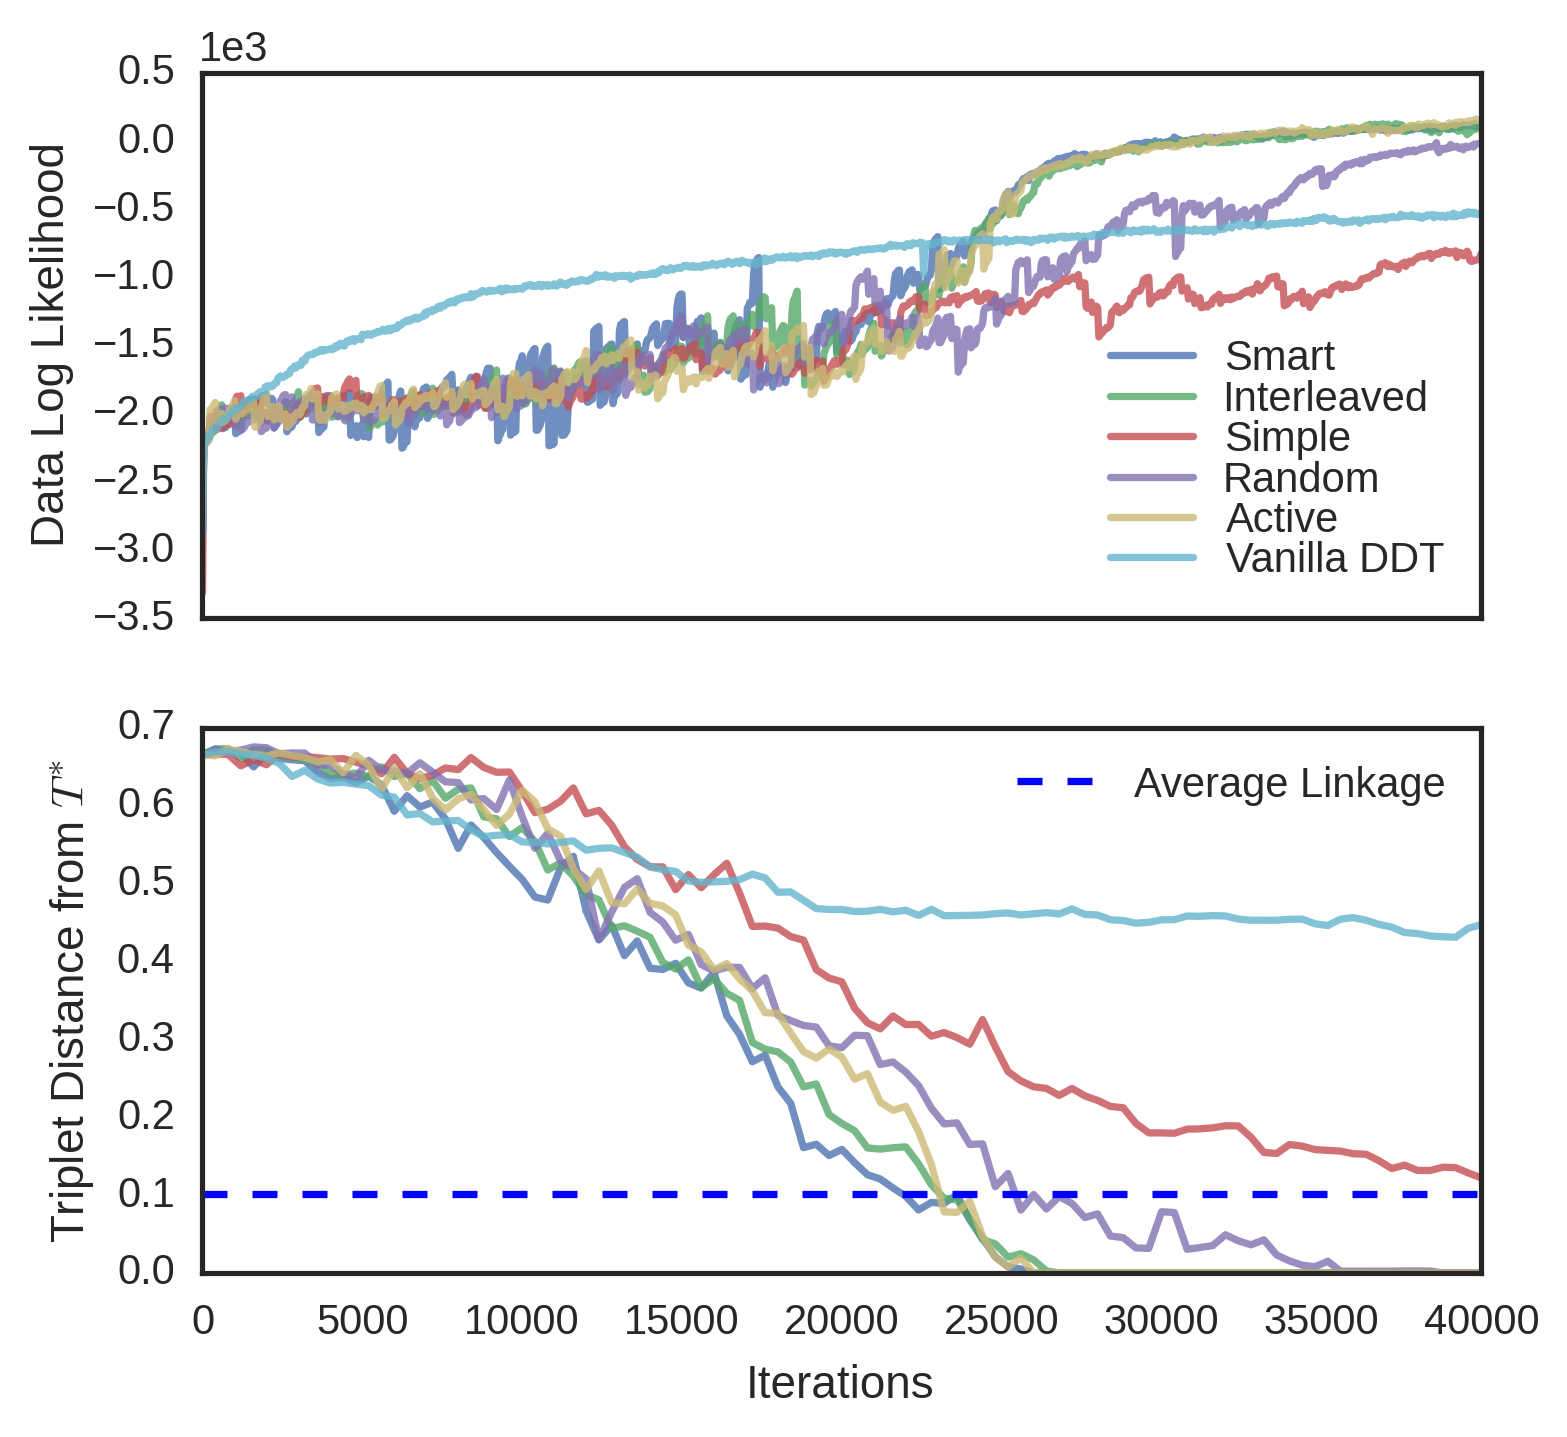
\includegraphics[width=\textwidth]{img/ibhc/Fisher-Iris-result.png} \caption{Fisher Iris}
        \label{fig:iris-result}
    \end{subfigure}
    \\
    \begin{subfigure}[]{0.7\textwidth}
        \centering
        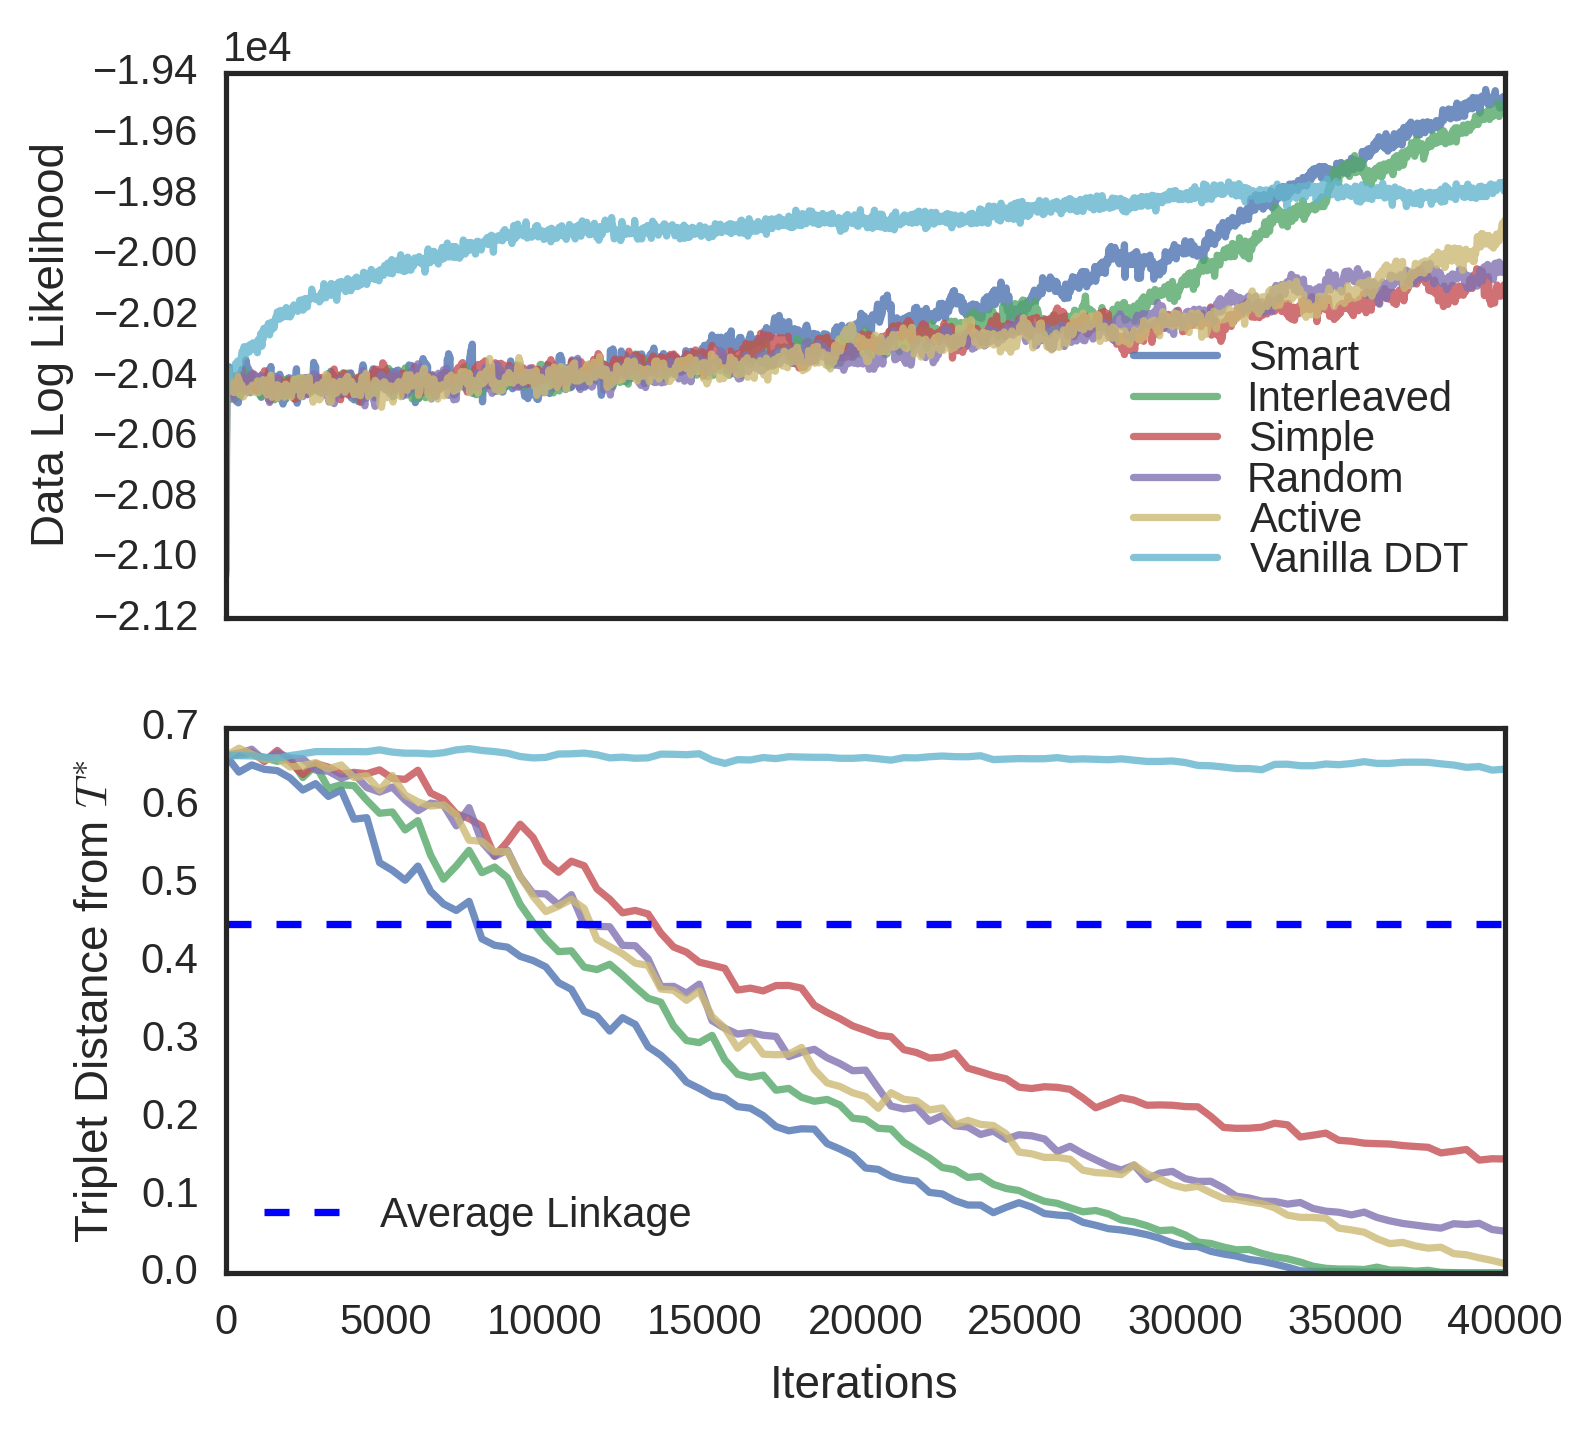
\includegraphics[width=\textwidth]{img/ibhc/MNIST-result.png}
        \caption{MNIST}
        \label{fig:mnist-result}
    \end{subfigure}
    \caption{The average of four runs of constrained-SPR samplers
    for the Fisher Iris dataset and the MNIST dataset, using 5 different querying schemes. A query was made every 100 iterations.}
    \label{fig:main-results}
\end{figure}

We evaluated the convergence properties of five different querying schemes.
In a ``simple query'', a user is presented with three random data
and picks an odd one out.
In a ``smart query'', a user is unrealistically shown the entire candidate tree and reports a violated triplet.
In a ``random query'', the user is shown the induced candidate tree over
a random subset of the data.
In an ``active query'', the user is shown a high variance 
subtree using tree-distance variance.
Finally, in an ``interleaved query'', the user is alternatively shown a random
subtree and a high variance subtree.
In each experiment, $\tree^*$ was known, so user queries were simulated
by picking a triplet
violated by the root split of the queried tree, 
and if no such triplet existed, recursing on a child.
%\begin{enumerate}
%\item Simple querying: a user is presented with three random data and
%reports a triplet of the data that should be satisfied.
%\item Smart querying (unrealistic): a user is presented with the entire tree
%and reports a triplet that is violated.
%\item Random querying: the user is shown the induced subtree
%over a random subset of the data of constant size
%and reports a violated triplet.
%\item Active querying: the user is shown a high variance
%induced subtree, chosen from a set of random subsets of data $\{S_1, \ldots , S_L\}$,
%with variance defined as tree distance variance. The user then reports
%a violated triple from this induced subtree.
%\item Interleaved querying: we alternate performing a random query
%and an active query.
%\end{enumerate}
Each scheme was evaluated on four different datasets.
The first dataset, MNIST \citep{MNIST}, is an 10-way image classification
dataset where the data are 28 x 28 images of digits.
The target tree $\tree^*$ is simply the $K$-way classification 
tree over the data.
The second dataset is Fisher Iris, a 3-way flower
classification problem, where each of 150 flowers has
five features.
The third dataset, Zoo ~\citep{Lichman2013}, is a set of 93 animals
and 15 binary morphological features for each of animals,
the target tree being the induced binary tree 
from the Open Tree of Life ~\citep{Hinchliff2015}.
The fourth dataset is 20 Newsgroups ~\citep{Joachims1997}, a
corpus of text articles on 20 different subjects. We use
the first 10 principal components as features
in this classification problem.
All datasets were modeled with DDT's with
acquisition function $a(t) = 1/(1 - t)$
and Brownian motion parameter $\sigma^2$ estimated from data.
To better visualize the different convergence rates
of the querying schemes, MNIST and  20 Newsgroups were subsampled
to 150 random points.

For each dataset and querying scheme, we instantiated a SPR
sampler with no constraints. Every one hundred iterations of the 
sampler, we performed a query.
In subtree queries, we used subsets of size $|S| = 10$ 
and in active querying, the highest-variance subset was chosen from $L = 20$ different random subsets.
As baselines,
we measured the triplet distance of the vanilla DDT
and the average linkage tree.
Finally, results were averaged over four runs of each sampler.
The triplet distances for Fisher Iris and MNIST can be seen in \autoref{fig:main-results}. Results for the other datasets
can be found in the supplement.
Although unrealistic due to the size of the tree shown to the user, 
the smart query performed the best, achieving minimum error
with the least amount of queries. Interleaved followed next,
followed by active, random, and simple. In general, the vanilla
DDT performed the worst, and the average linkage
score varied on each dataset, but in all cases, the
subtree querying schemes performed better than both the vanilla DDT
and average linkage.

In three datasets (MNIST, Fisher Iris and Zoo), 
interactive methods
achieve higher data likelihood than the vanilla DDT.
Initially, the sampler is often restructuring the tree
with new triplets
and data likelihood is unlikely to rise. However, over time
as less triplets are reported,
the data likelihood increases rapidly.
We thus conjecture that triplet constraints 
may help the MH algorithm find better optima.

\section{Future Work}
We are interested in studying the non-realizable case, i.e.
when there does not exist a tree that satisfies triplet set $C$. We would also like to better understand the effect of constraints on searching
for optima using MCMC methods.
